\chapter{Multi-directional Waves}
\label{chap:MultiDir}


In order to incorporate bi-directional waves, changes were made to the input files, how the data is stored internally, and to the computation of the first order forces. The second order forces were designed from the beginning to include bi-directional waves.

For our implimentation of the multi-directional waves, we are using the equal energy discretization which is used in the commercial code OrcaFlex.  With this method the same $N/2+1$ frequencies as used in the uni-directional case are used here.  A total of $\Theta$ (\varname{WaveNDir} in input file) discrete directions are used and each frequency is assigned to one of the discrete directions.
The value of $(\frac{N}{2}) / \Theta$ needs to be an integer so that each direction contains the same number of frequencies. $\Theta$ may need to be adjusted within the \modname{Waves} module to ensure this is true (see \Cref{sec:MultiDir:ThetaAdjust}).

\begin{center}
   \begin{minipage}[t]{\linewidth}
      \fvset{frame=single,fontsize=\scriptsize,numbers=left,numbersep=3pt,obeytabs,tabsize=1,fontfamily=fvm,commentchar=\%}
      \VerbatimInput{chaps/HD_Input/HD_Input_File_Waves.txt}
   \end{minipage}
   \captionof{table}{New section for the \HD input file for multi-directional waves.  This section is inserted where \emph{WaveDir} is currently defined.}
   \label{tab:HD_WAMIT2_InputModsWaveDir}
\end{center}


If $\varname{WaveDirMod}=1$, then a check is performed to make sure that $\varname{WaveMod}=$2, 3, or 4 (JONSWAP, white-noise, user defined).  If this is true, then an internal logical variable \varname{WaveMultiDir} is set to true and passed to modules that need to know about multiple wave directions.

Within the code in the \modname{HydroDyn\_Input} module, the maximum and and minimum directions actually used stored as \varname{WaveDirMin} and \varname{WaveDirMax}.  Since the wave direction assignments are performed using the equal energy approach, the actual maximum and minimum values will cover a smaller range than requested by the \varname{WaveDirRange} variable (see \Cref{sec:MultiDir:Testing}).
\begin{eqnarray}
   \varname{WaveDirMin} >& \varname{WaveDir} - \varname{WaveDirRange}/2\\
   \varname{WaveDirMax} <& \varname{WaveDir} + \varname{WaveDirRange}/2.
\label{eq:WaveDirMinMax}
\end{eqnarray}
These variables will be used in checking the WAMIT output files used (both first and second order).  Care should be taken to allow for crossing the $\pm \pi$ direction boundary.


\section{Adjusting $\Theta$ within the \modname{Waves} module}
\label{sec:MultiDir:ThetaAdjust}
To use the equal energy approach outlined below, $(\frac{N}{2}) / \Theta$ must be an integer, so it may be necessary to change $\Theta$ from the user specified value.  The difficulty with enforcing this arises from three requirements:
\begin{enumerate}
   \item{WaveNDir is odd in order to keep the center direction}
   \item{$N$ is adjusted by HydroDyn to be a product of smallish numbers for efficiency in the FFT\label{list:N}}
   \item{$(\frac{N}{2})/\Theta$ needs to be an integer to keep the energy distribution correct\footnote{Originally the requirement was set such that $(\frac{N}{2}-1)/\Theta$ was used (the $\omega=0$ frequency was ignored).  However, it was found that $(\frac{N}{2}-1)/\Theta$ was often a prime number, which would lead to user frustration.}}
\end{enumerate}
The third requirement means that $N/2$ is a product of integers such that $\Theta$ is one of them.  For small values of $\Theta$, this is unlikely to be an issue when $N$ is large, but could be problematic for short simulations where $N$ is smaller.\footnote{$N$ is initially set to \varname{TMax}/\varname{WaveDT} and then increased until it is the product of small numbers.}  For large values $\Theta$, it becomes less likely this would be true.  In order to satisfy these conditions, the value of $\Theta$ will be adjusted.\footnote{While it is theoretically possible to adjust $N$ such that the third condition is satisfied, this would have the undesirable consequence of changing the frequency step (see \Cref{eq:IFFT_N}).  This would in turn change the values of the complex wave amplitude in frequency space ($A_m$) for a given random number seed value.  Subsequently, the ability to reproduce the wave height and wave force timeseries for a given seed pair would not be preserved.}

For small values of $\Theta$, it may only be necessary to increase it slightly to satisfy the requirements (for example, change $\Theta=7$ to $\Theta=9$).  For large values of $\Theta$ (perhaps $>60$), it may be necessary adjust the value several times before a suitable value is found.  This could be done as outlined in \Cref{fig:Theta:Adjust}.  Note that we do not want to simply allow $\Theta$ to increase until a suitable value is found in the unlikely event that $N/2$ is a prime number.  In this case $\Theta$ will have to be increased until $\Theta=N/2$, which would mean each frequency has a unique wave heading and no binning occured.  This can only be corrected by having the user change \varname{WaveDT} or \varname{WaveTMax} since $N$ is adjusted internally to satisfy condition \ref{list:N}.
\begin{figure}
   \centering\begin{tikzpicture}

% Init
\node[process,text width=35mm] 
      (initialize)  {$\Theta_{init}=\Theta$\\ 
                     $\Theta_\text{max}=1.25\times \Theta_\text{init}$};

% odd?
\node[decision,below of=initialize,node distance=20mm]
      (odd) {Is $\Theta$ odd};
   \draw[cl] (initialize.south) -- (odd);

  % n branch
   \node[process,right of=odd,node distance=35mm,text width=25mm]
         (makeodd) { $\Theta=\Theta+1$\\
                     $\Theta_{init} = \Theta$\\
                     Warn user that it wasn't odd and new value.};
      \draw[cl] (odd) -- (makeodd) node[midway,above] {n};


% first check, continue
\node[decision,below of=odd,node distance=20mm,text width=20mm,inner sep=0pt]
      (CheckTheta1) {$(\frac{N}{2})/\Theta$\\integer};
   \draw[cl] (odd) -- (CheckTheta1) node[midway,left] {y};
   \draw[cl] (makeodd) -- (CheckTheta1);

   %y branch, done
   \node[process,text width=20mm]
         (Done1) at ($(CheckTheta1 -| makeodd)$)  {No change to $\Theta$};
      \draw[cl] (CheckTheta1) -- (Done1) node[midway,above] {y};
   % return
   \node[return,right of=Done1,node distance=25mm]
         (Return1) {Return};
      \draw[cl] (Done1) -- (Return1);

% not done, search up for solution
\node[process,below of=CheckTheta1,node distance=20mm]
      (Increase) {$\Theta=\Theta+2$};
   \draw[cl] (CheckTheta1) -- (Increase) node[midway,left] {n};

\node[decision,below of=Increase,node distance=20mm,text width=20mm,inner sep=0pt,font=\footnotesize]
      (ThetaLimitUpper) {$\Theta < \Theta_\text{max}$};
   \draw[cl] (Increase) -- (ThetaLimitUpper);

   % if still within range, check value
   \node[decision,right of=ThetaLimitUpper,node distance=45mm,text width=20mm,inner sep=0pt]
         (CheckTheta2) {$(\frac{N}{2})/\Theta$\\integer};
      \draw[cl] (ThetaLimitUpper) -- (CheckTheta2) node[midway,above] {y};

   % if we have an answer, done and return.  If not, loop again
   \node[process,right of=CheckTheta2,node distance=40mm,text width=25mm]
         (Finish) {Tell user what $\Theta$ is and why};
      \draw[cl] (CheckTheta2) -- (Finish) node[midway,above] {y};
      % Return
      \node[return,right of=Finish,node distance=25mm]
            (Return2) {Return};
         \draw[cl] (Finish) -- (Return2);
      % or loop again
      \draw[cl] (CheckTheta2) |- (Increase) node[midway,below left] {n};

%%% --- Don't go down.  We only want to increase resolution, not decrease it.
%% didn't find solution before getting too big
%\node[process,below of=ThetaLimitUpper,node distance=20mm]
%      (Decrease) {$\Theta=\Theta_{init}-2$};
%   \draw[cl] (ThetaLimitUpper) -- (Decrease) node[midway,left] {n};
%
%\node[decision,below of=Decrease,node distance=20mm,text width=20mm,inner sep=0pt,font=\footnotesize]
%      (ThetaLimitLower) {$\Theta > \Theta_{init} \cdot (1.0-\Delta\Theta_\text{allow})$};
%   \draw[cl] (Decrease) -- (ThetaLimitLower);
%
%   % if still within range, check value
%   \node[decision,text width=20mm,inner sep=0pt]
%         (CheckTheta3) at ($(ThetaLimitLower)!.5!(ThetaLimitLower -| CheckTheta2)$) {$(\frac{N}{2})/\Theta$\\integer};
%      \draw[cl] (ThetaLimitLower) -- (CheckTheta3) node[midway,above] {y};
%      % if we do have an answer, retun
%      \draw[cl] (CheckTheta3) -| (Finish) node[midway,above left] {y};
%      % if not, loop again
%      \draw[cl] (CheckTheta3) |- (Decrease) node[midway,below left] {n};

% exceeded limit before finding solution
\node[process,below of=ThetaLimitUpper,node distance=27mm,text width=40mm]
      (NoSolution) {No Solution in range:\\$\Theta_\text{init} \rightarrow \Theta_\text{max}$\\Try changing $\Theta$ or \varname{WaveTMax}};
   \draw[cl] (ThetaLimitUpper) -- (NoSolution) node[midway,left] {n};

\node[return,right of=NoSolution,node distance=60mm,text width=40mm]
      (Return3) {Fatal Error: Return suggested value of WaveNDir if exists};
   \draw[cl] (NoSolution) -- (Return3);




\end{tikzpicture}
\endinput



\end{tikzpicture}
\endinput

%inputs from file
\node[process,below of=p1]
      (p2)  {Read input from file (and check)};
   \draw[cl] (p1) -- (p2);
   \draw[cl] (p2.south west) .. controls +(-4mm,-4mm) and +(-4mm,4mm) .. (p2.north west) node[midway,sloped,above,yshift=-1mm,font=\scriptsize] {NumCases};

% return
\node[return,below of=p2] (r1) {Return};
   \draw[cl] (p2) -- (r1);

\end{tikzpicture}

   \caption[Flowchart of how to find a suitable value of $\Theta$]{Flowchart of how to find a suitable value of $\Theta$ such that $(\frac{N}{2})/\Theta$ is an integer.  The reason for suggesting that \varname{WaveTMax} should be changed is that there is a possibility that $N/2$ is a prime number.  This is implimented at the start of the initialization subroutine of the \modname{Waves} module if multidirectional waves are selected.\label{fig:Theta:Adjust}}  
\end{figure}
 



\section{Equal Energy Approach}
\label{sec:MultiDir:EqEnergy}


\begin{table}[H]
   \centering
   \caption[Notation for multi-directional wave equations]{Notation for multi-directional wave equations.\label{tab:MultiDirWaves:Notation}}
   \begin{tabular}{cclc}
      \toprule
         Variable                   &  Variable Name           &  Description                            &  Units    \\
      \midrule
         $\Theta$                   &  \varname{WaveNDir}      &  User defined number of wave directions &   -       \\
         $\theta$                   &                          &  Current wave direction                 &  degrees  \\
         $\bar\theta$               &  \varname{WaveDir}       &  Central (mean) wave direction          &  degrees  \\
         $\delta\theta$             &  \varname{WaveDirRange}  &  Range of wave directions (full width)  &  degrees  \\
         $S$                        &  \varname{WaveDirSpread} &  Spreading function coefficient (1 typ) &   -       \\
      \bottomrule
   \end{tabular}
\end{table}




This method to simulate multi-directional waves assigns each frequency component of the wave to one of $\Theta$ discrete wave directions.  Each wave direction will have the same number of frequencies, $(\frac{N}{2})/\Theta$, assigned to it.  In order to preserve the energy distribution in the wave spreading function, the wave directions are assigned so that a greater number of directions are concentrated near the central frequency.

This method is only valid if the equation describing the total spectrum is separable into the frequency and direction parts as follows:
\begin{equation}
   S(\omega,\theta) = \bar{S}(\omega) \cdot D(\theta).
\label{eq:totalspectrum}
\end{equation}

The wave spreading function is given by
\begin{equation}
   D(\theta)   = C \left| \cos\left(\frac{\pi \: (\theta - \bar\theta)}{\delta \theta}\right) \right|^{2S},
\label{eq:WaveSpread}
\end{equation}
where the normalization constant, $C$, is given by
\begin{equation}
   C = \frac{\sqrt{\pi} \: \Gamma(S+1)}{\delta\theta \: \Gamma(S+1/2)},
\label{eq:WaveSpread:Const}
\end{equation}
and $\Gamma$ is the gamma function.
The spreading function should satisfy the normalization condition of
\begin{equation}
   \int\limits^{\bar\theta+\delta\theta/2}_{\bar\theta-\delta\theta/2} D(\theta) \, \mathrm{d}\theta \equiv 1.
\label{eq:WaveSpread:Norm}
\end{equation}
The cumulative energy distribution within the wave spreading function up to angle $\theta$ is given by
\begin{equation}
   P(\theta) = \int\limits^{\theta}_{\bar\theta - \delta\theta/2} D(\theta') \: \mathrm{d}\theta'.
\label{eq:WaveSpread:Energy}
\end{equation}

The following method may be used to set the appropriate wave directions to satisfy the equal energy approach.
\begin{enumerate}
   \item{Discretize the wave direction range $\delta\theta$ by $n_d$ steps and calculate $D(\theta)$ spreading function.  Set $n_d$ to a sufficiently large number such that the function is smooth enough for interpolation over $\Theta$ directions (set $n_d = 3 \Theta$).\label{list:EqEnergySolve:1}}
   \item{While calculating $D(\theta)$, calculate the cumulative energy sum up to the current direction as $P(\theta)$.}
   \item{Discretize $P(\theta)$ into $\Theta$ steps from $1/\Theta \leq P_i \leq 1-1/\Theta$.  Interpolate the function $D(\theta)$ found in step \ref{list:EqEnergySolve:1} to find the corresponding values of $\theta_i$.  The $\theta_i$ values are the wave directions used in the equal energy method.}
   \item{Randomly assign each of the $N/2$ frequencies (ignoring the end frequencies at which the wave amplitude is defined as zero) to a $\theta_i$ direction such that each wave direction has $(N/2)/\Theta$ frequencies assigned to it. \emph{This is the tricky bit to do such that the assignments are the same given a certain random number seeed pair.}}   % randomly assign to wave bins in groups of \Theta frequency sets.
\end{enumerate}

\subsection{A few notes}
There are a few things to take note of in this process.  First, in order to preserve the equal energy distribution within the wave direction spreading function, care must be taken so that $(N/2)/\Theta$ is an integer (see \Cref{sec:MultiDir:ThetaAdjust} for caveats with using a user defined value for $\Theta$).  Second, if it is desirable to have a greater number wave directions, it is preferable to increase $\Theta$ substantially.  Alternatively, the $\theta_i$ values could be treated as wave direction bins spanning a range of $\theta$ directions rather than a single direction.  The danger with this is that the distribution of random wave directions within the bin will affect the overall energy distribution of the spreading function.  A shaping function would then need to be applied to the bin to distribute wave directions within it.  In this case it would be preferable to increase $\Theta$ significantly in order to allow for more wave directions while preserving the energy distribution in the wave spreading function.  Short tests using MATLAB code indicate that a value of $\Theta = 399$ works well for allowing a seemingly random set of wave directions.  In practice, it may be preferable to keep $\Theta < 50$ for a more physical description of wave directionality.

%NOTE: there is a discrepency between this approach and what OrcaFlex does.  See page 155 of the version 9.7a manual.  In the OrcaFlex approach, the wave amplitude is held constant, and the frequency spacing is changed so as to preserve the energy content on the amplitude vs. frequency spectrum.  Our implimentation is slightly different in that we have a uniform $\Delta\omega$ and vary the amplitude.

\subsection{Implimentation and Testing}
\label{sec:MultiDir:Testing}

\paragraph*{Development testing}
During the implimentation of the multidirectional waves within the \modname{Waves} module, testing was performed to ensure that no errors were introduced into the equations used to calculate the wave elevation, velocity, and acceleration.  The following sequence was used to impliment the multidirectional waves within the waves module.
\begin{enumerate}
   \item{Add code section to change the value of \varname{WaveNDir}.  This was originally implimented such that $(\frac{N}{2}-1)/\Theta$ was an integer.  This was later changed when it was discovered that $(\frac{N}{2}-1)$ is often a prime number (due in part to how \varname{NStepWave} is adjusted -- see \Cref{sec:MultiDir:ThetaAdjust} for details). This code was tested before proceeding.}
   \item{Split the main loop over \varname{NStepWave2} frequencies.  The wave direction assignment loop is inserted between the first loop where the wave amplitudes and phases are assigned, and the second loop where the IFFTs are setup and performed.  Testing was performed to ensure that all the information necessary in the second loop existed.}
   \item{Create the wave direction assignment loop.  Some temporary print statements were used to output the wave direction information for plotting.  These results are shown in \Crefrange{fig:MultiDir:WavesTest001}{fig:MultiDir:WavesTest008}.}
   \item{The code necessary for processing the input array \varname{WaveElevXY} and return array \varname{WaveElevSeries} was developed at the \modname{Waves} module and the \modname{WAMIT2} driver level.  The subroutine for calculating the wave elevation at a specified $(x,y)$ coordinate was developed.  Movies were then created of the test cases listed in \Cref{tab:MultiDir:Tests} to verify that the wave elevation calculations were working correctly (it too some iterating to get this working).}
   \item{The code was then rearranged and modified so that the \varname{WaveElevXi}, \varname{WaveElevYi} elevation data uses the wave elevation routine.}
   \item{Now the wave velocity and acceleration equations were modified.  In the original calculations, the wave direction was handled after the FFT.  This was revised so that the wave direction was handled before the FFT was calculated.  Testing of this was performed by setting \varname{WaveNDir} = 1 and repeating a few CertTests that had been generated with the previous version of the \modname{Waves} module.  The results agreed to within the precision used for outputting the CertTest results.}
\end{enumerate}

At this point, it was concluded that the \modname{Waves} module was working as well as it had been prior to the implimentation of multi-directional waves.  A minor usability issue became apparent at this point regarding how \varname{WaveNDir} was adjusted within the code.  The decision was then made to modify the code such that we include the $\omega = 0$ term in the wave direction assignment.  This means that we now force $(\frac{N}{2})/\Theta$ to be an integer.  We also included code to give the user some idea of what values of \varname{WaveNDir} might work with their currently defined values of \varname{WaveTMax} and \varname{WaveDT}.

For testing the multi-directional waves there is one more test we can perform.  This is to check the correlation of the wave elevation at various $(x,y)$ locations.  This has not been performed yet.\todo{do this}



\paragraph*{Test Cases}
Multidirectional waves using the method described above are implimented within the \modname{Waves} module of \HD.  It is evaluated after the generation of the wave spectrum (JONSWAP or other).  The directions are assigned in groups of $\Theta$ frequencies so that one each frequency within the group is assigned a unique direction.  This is repeated for all $(N/2)/\Theta$ groups of frequencies.

Several test cases were performed to verify that the assignment of wave directions by frequency was correctly performed.  In each of the test cases listed in \Cref{tab:MultiDir:Tests}, a compiled version of the code with partially implimented modifications to the \modname{Waves} module was executed.  The calculated spreading function, integrated power of the spreading function, calculated wave directions, and the assigned wave directions were output using appropriately placed print statements (this was merely intended as an intermediate testing of the code, not a test that would be needed in this form later).  The results were plotted using gnuplot.

Tests numbered 002 and 004 are very similar with the only differences in $\bar\theta$, the mean wave direction, and $S$, the spreading coefficient.  A comparison of \Cref{fig:MultiDir:WavesTest002} and \Cref{fig:MultiDir:WavesTest004} shows the repeatablility during the assignment of the wave direction for each frequency: in each test, the $n^\text{th}$ frequency is assigned to the same wave direction index.  Though the frequencies are randomly assigned, the same seed was used in each of these tests and the random number generator had the same number of calls for wave amplitude prior to the assignment of the directions.

Tests numbered 001, 005, and 008 are identical with the exception of the mean wave direction.  Test 001 is oriented with the mean wave direction along the $x$ axis, and test 005 is oriented with the mean wave direction along the positive $y$ axis.  A movie of the sea surface for these two tests is useful in checking that the coordinate transformations are working correctly.

\begin{table}
   \centering
   \caption[Multi-directional waves test cases]{Multi-directional waves test case parameters.\label{tab:MultiDir:Tests}}
%   \tabcolsep=1.75mm
   \begin{tabular}{cccccccccc}
      \toprule
 Test Case  & \varname{WaveDirMod}&$\bar\theta$ &  $\delta\theta$ &  $S$   &  $\tau_\text{max}$ &  $\Delta\tau$   &  $N/2$ &  $\Theta$ &  $\frac{N/2}{\Theta}$  \\
  (-)       &                 &  (deg)          &  (deg)          &  (-)   &  (s)               &  (s)            &  (-)   &  (-)      &  (-)                     \\
      \midrule
   001      &      1          &    0            &   50            &  1.0   &   85               &  0.25           &  170   &  17       &  10                      \\
   002      &      1          &   45            &   60            &  1.0   &  150               &  0.25           &  300   &  25       &  12                      \\
   003      &      1          & -137            &   45            &  1.0   &  390               &  0.25           &  780   &  39       &  20                      \\
   004      &      1          &  135            &   45            &  2.3   &  150               &  0.25           &  300   &  25       &  12                      \\
   005      &      1          &   90            &   50            &  1.0   &   85               &  0.25           &  170   &  17       &  10                      \\
   006      &      0          &   45            &   60            &  1.0   &  150               &  0.25           &  300   &  --       &  --                      \\
   007      &      0          & -137            &   45            &  1.0   &  390               &  0.25           &  780   &  --       &  --                      \\
   008      &      1          &   15            &   35            &  1.0   &   85               &  0.25           &  170   &  17       &  10                      \\
      \bottomrule
   \end{tabular}
\end{table}


\begin{figure}
   \centering
   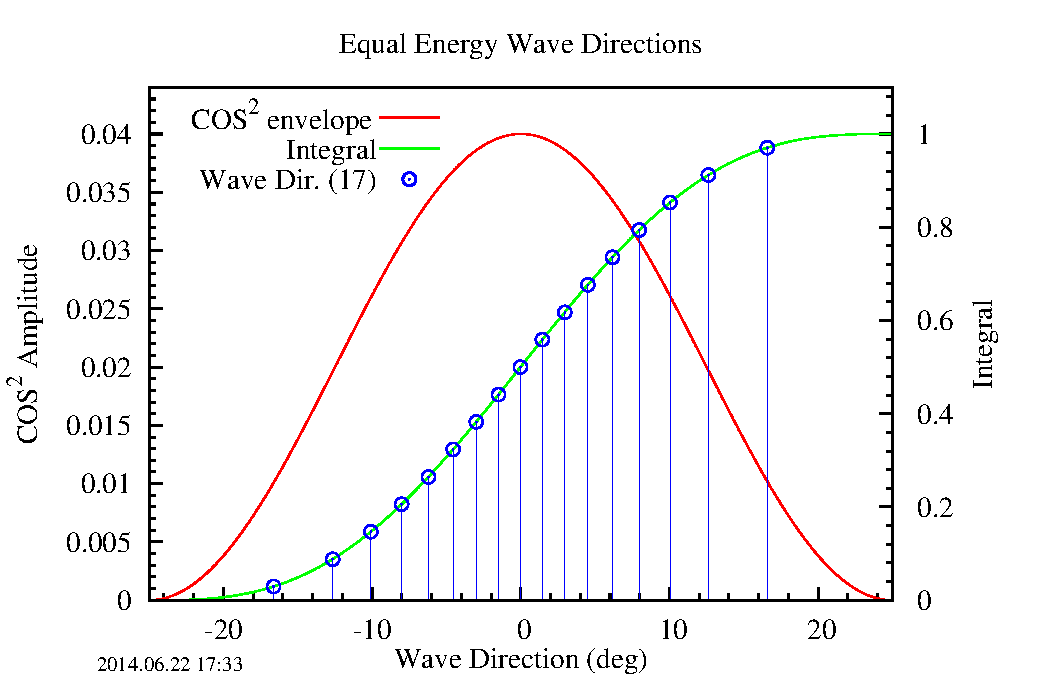
\includegraphics[width=.47\linewidth]{chaps/figures/WaveDirTest/WavesTest_001--equal_energy_disc.pdf}
   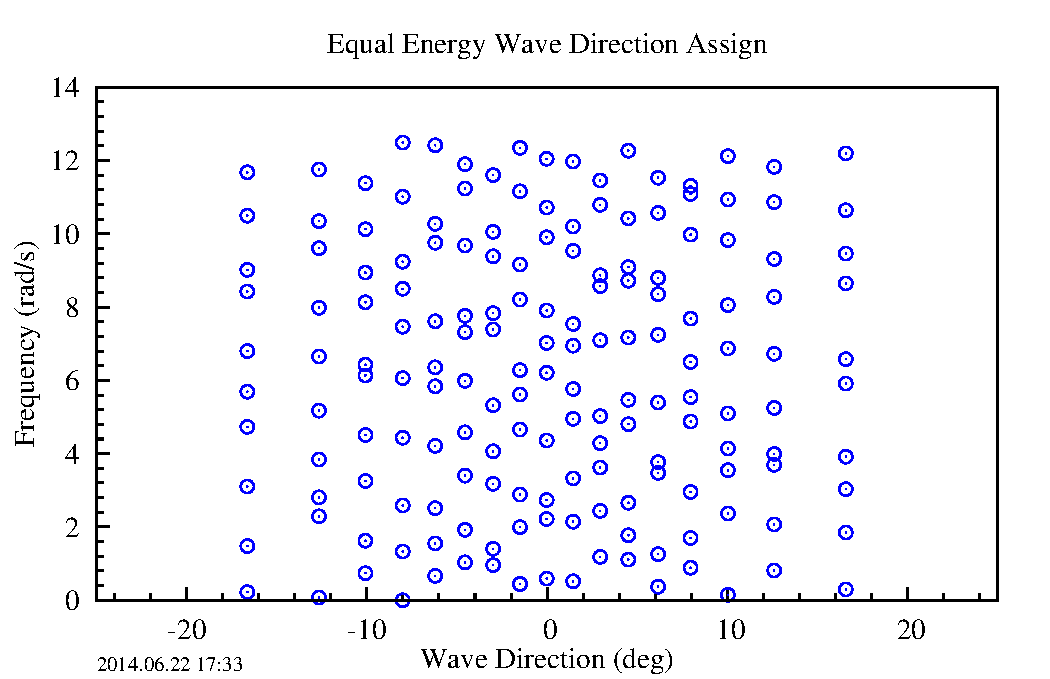
\includegraphics[width=.47\linewidth]{chaps/figures/WaveDirTest/WavesTest_001--wavedir_assign.pdf}
   \caption{Test case 001.  The right plot shows the randomly selected directions for each frequency.\label{fig:MultiDir:WavesTest001}}
\end{figure}

\begin{figure}
   \centering
   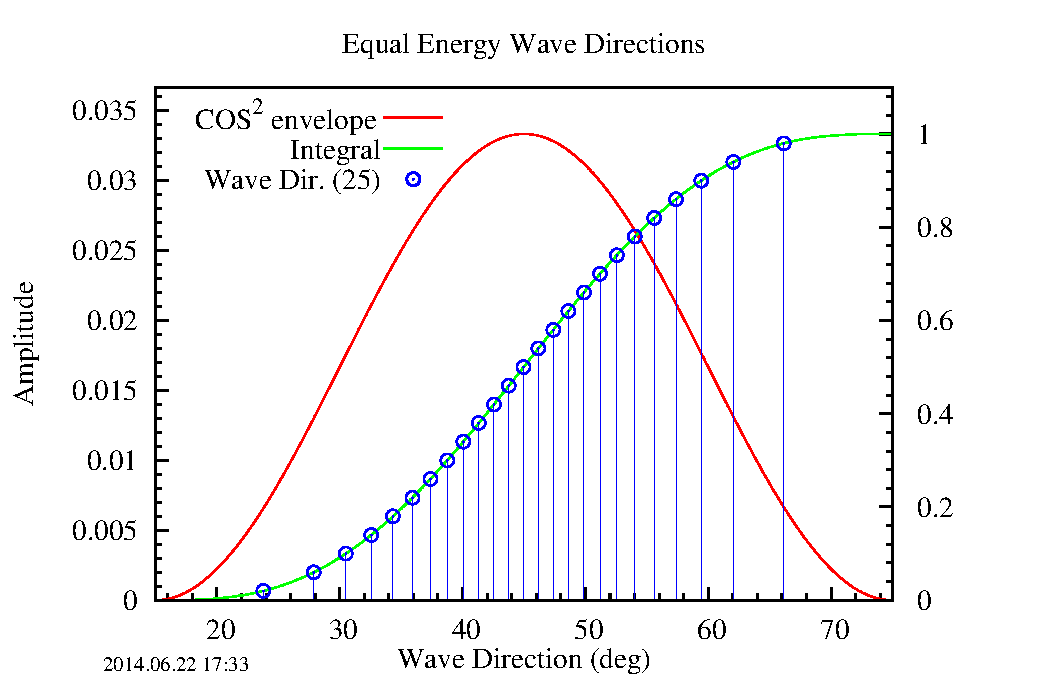
\includegraphics[width=.47\linewidth]{chaps/figures/WaveDirTest/WavesTest_002--equal_energy_disc.pdf}
   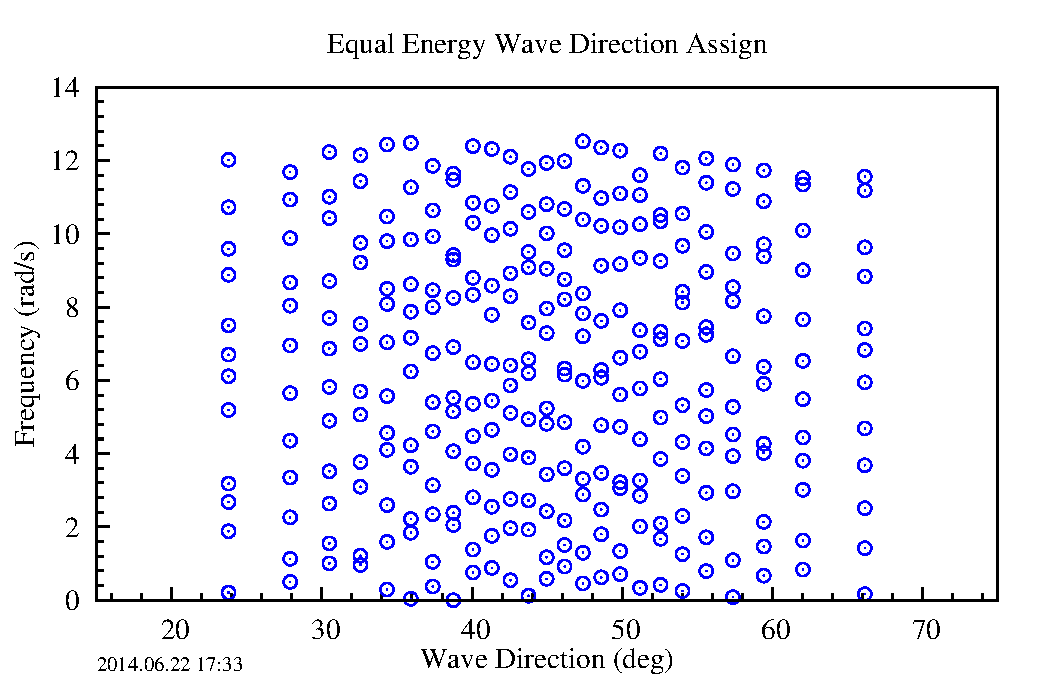
\includegraphics[width=.47\linewidth]{chaps/figures/WaveDirTest/WavesTest_002--wavedir_assign.pdf}
   \caption{Test case 002.  The right plot shows the randomly selected directions for each frequency.\label{fig:MultiDir:WavesTest002}}
\end{figure}

\begin{figure}
   \centering
   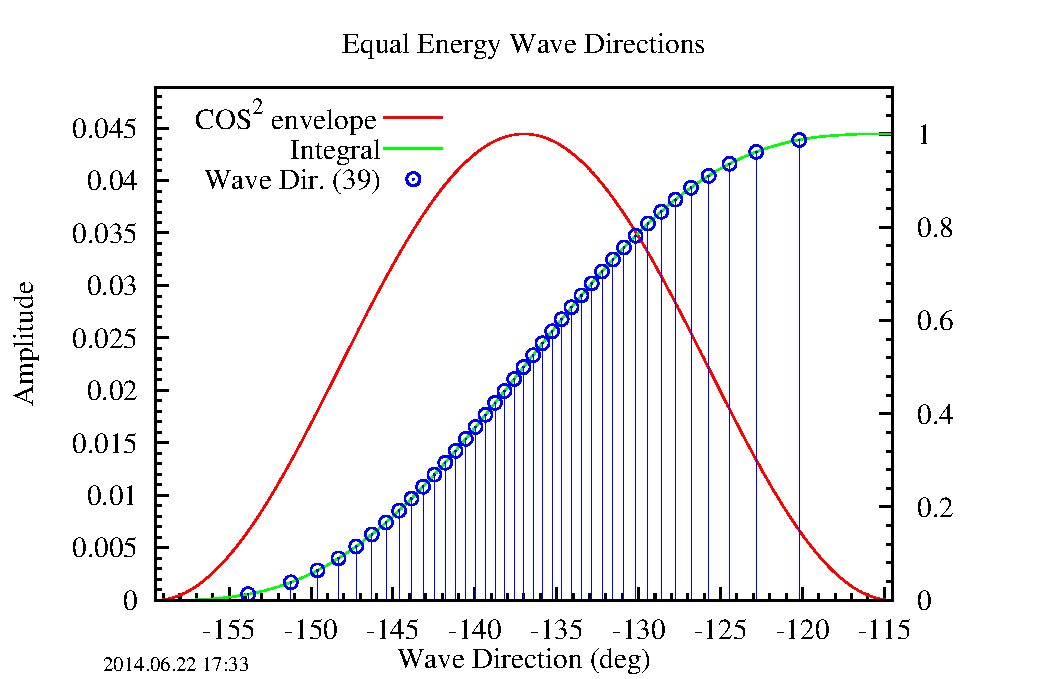
\includegraphics[width=.47\linewidth]{chaps/figures/WaveDirTest/WavesTest_003--equal_energy_disc.pdf}
   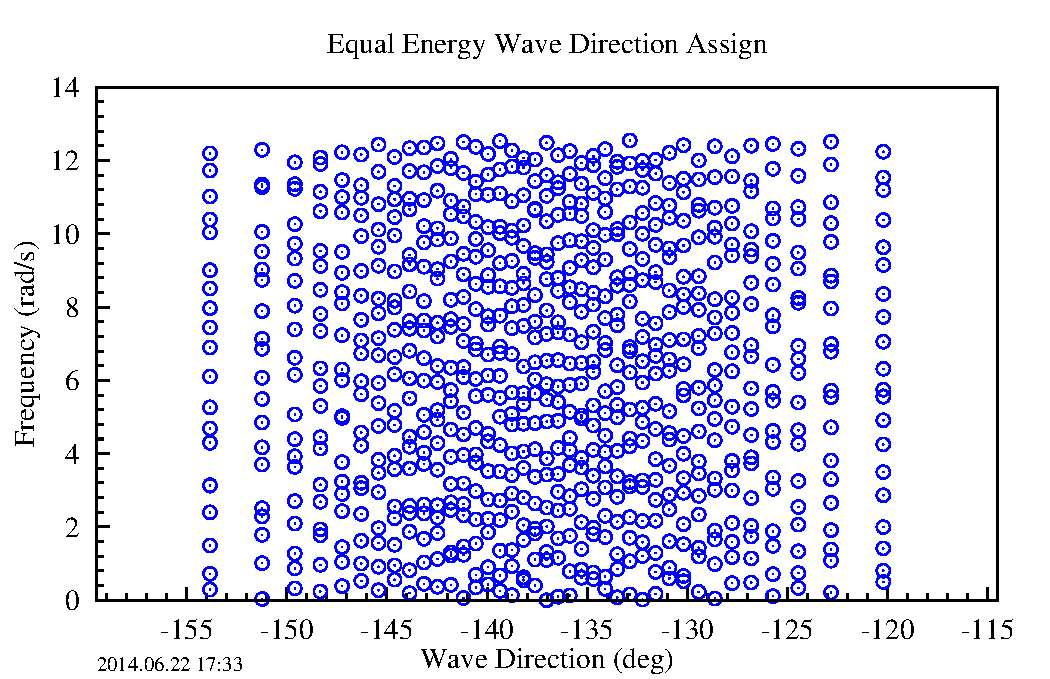
\includegraphics[width=.47\linewidth]{chaps/figures/WaveDirTest/WavesTest_003--wavedir_assign.pdf}
   \caption{Test case 003.  The right plot shows the randomly selected directions for each frequency.\label{fig:MultiDir:WavesTest003}}
\end{figure}

\begin{figure}
   \centering
   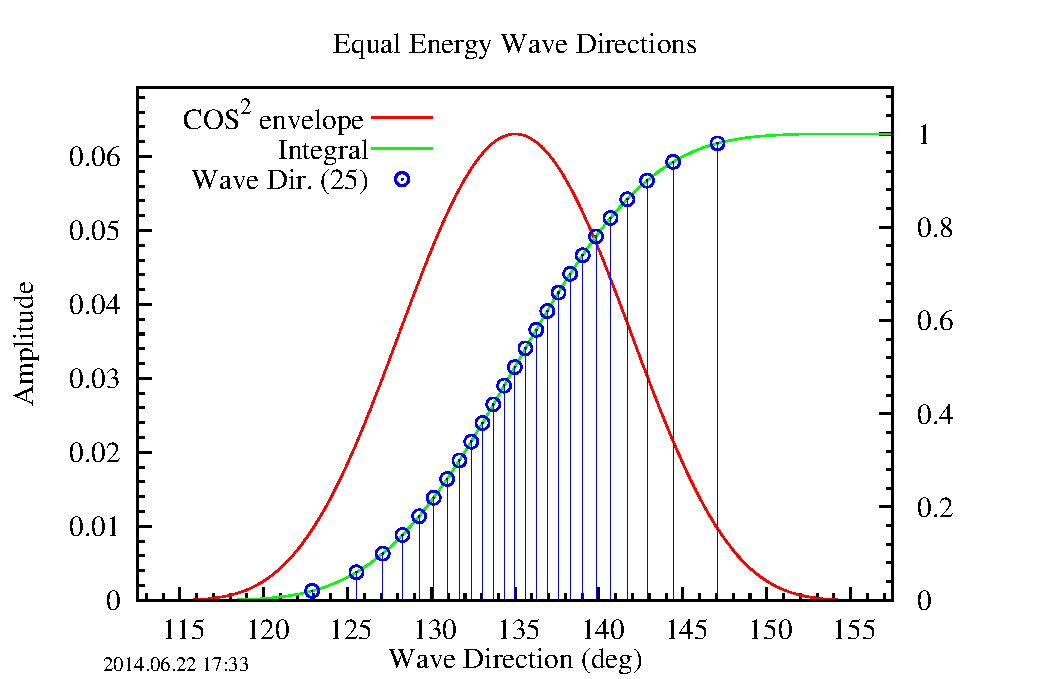
\includegraphics[width=.47\linewidth]{chaps/figures/WaveDirTest/WavesTest_004--equal_energy_disc.pdf}
   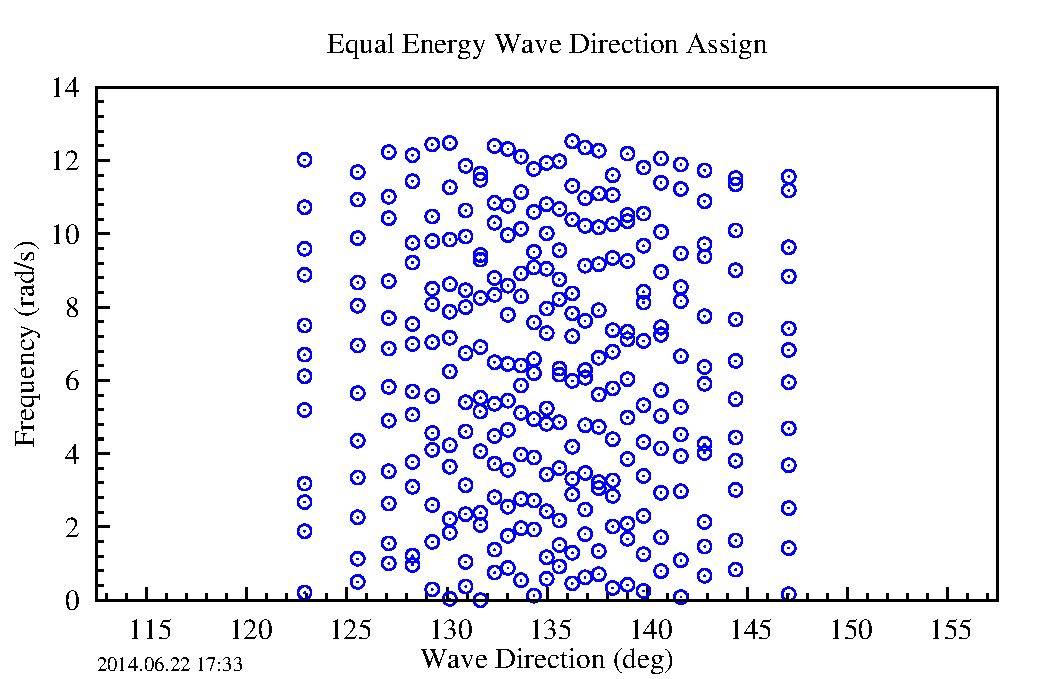
\includegraphics[width=.47\linewidth]{chaps/figures/WaveDirTest/WavesTest_004--wavedir_assign.pdf}
   \caption{Test case 004.  The right plot shows the randomly selected directions for each frequency.  This is the same as test case 002 with $\bar\theta=135$ and $S=2.3$.  Note that the ordering of the assigned frequencies is the same as in case 002.\label{fig:MultiDir:WavesTest004}}
\end{figure}

\begin{figure}
   \centering
   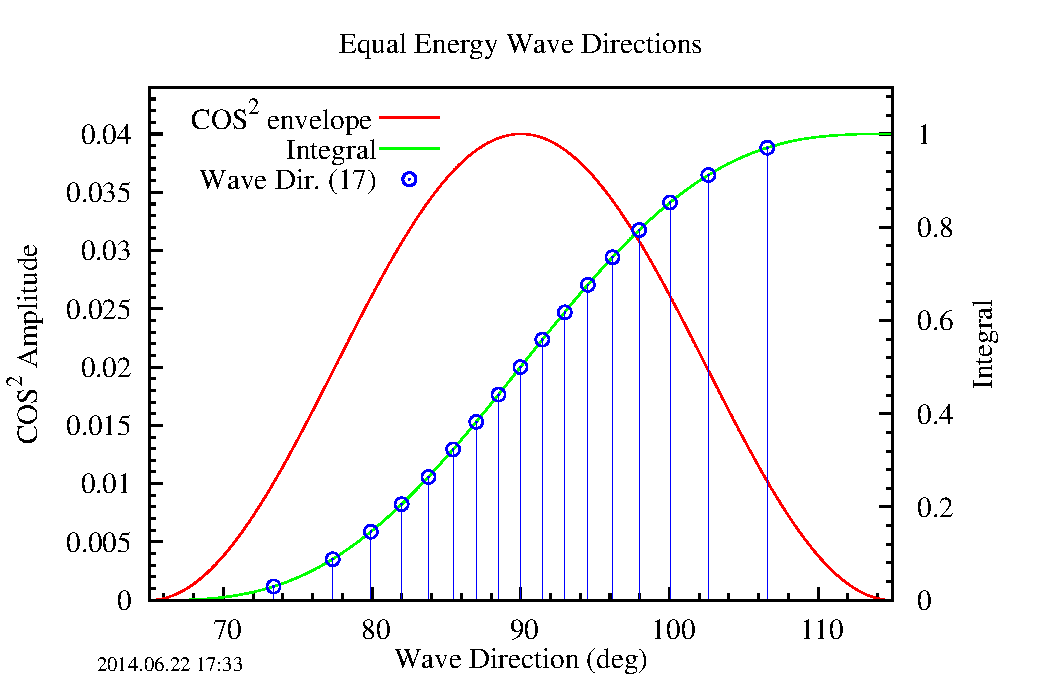
\includegraphics[width=.47\linewidth]{chaps/figures/WaveDirTest/WavesTest_005--equal_energy_disc.pdf}
   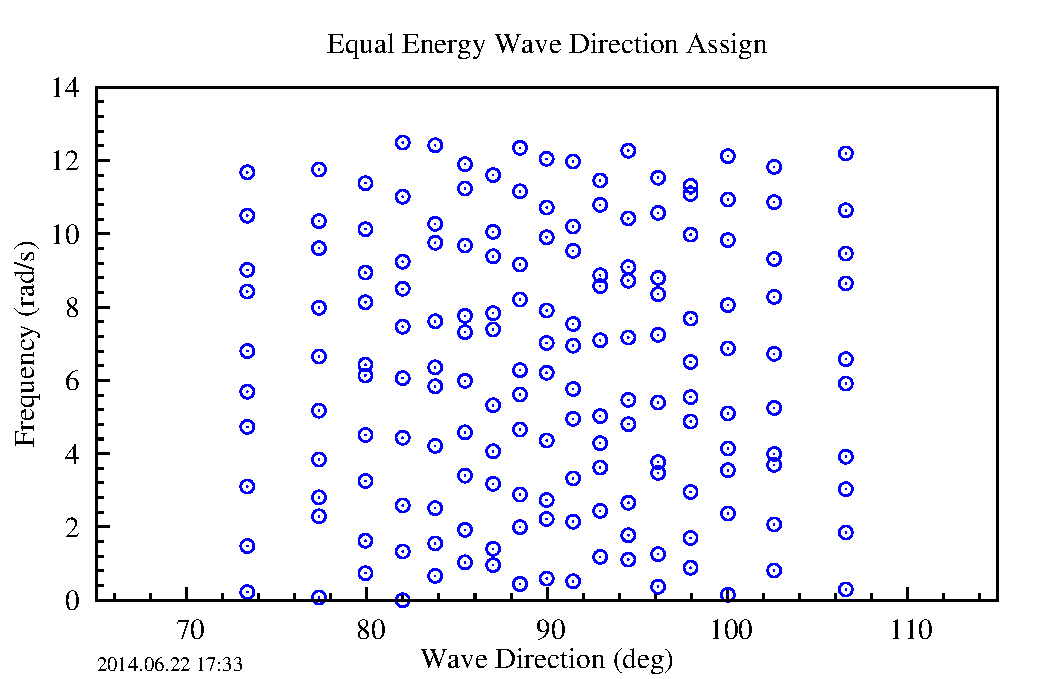
\includegraphics[width=.47\linewidth]{chaps/figures/WaveDirTest/WavesTest_005--wavedir_assign.pdf}
   \caption{Test case 005.  The right plot shows the randomly selected directions for each frequency.\label{fig:MultiDir:WavesTest005}}
\end{figure}

\begin{figure}
   \centering
   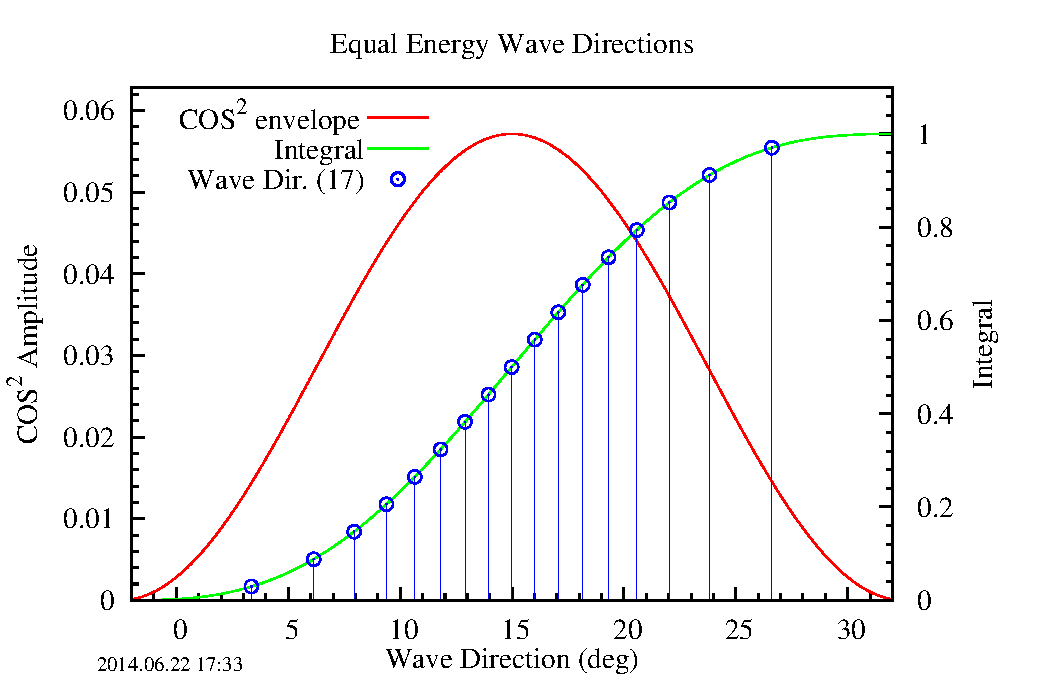
\includegraphics[width=.47\linewidth]{chaps/figures/WaveDirTest/WavesTest_008--equal_energy_disc.pdf}
   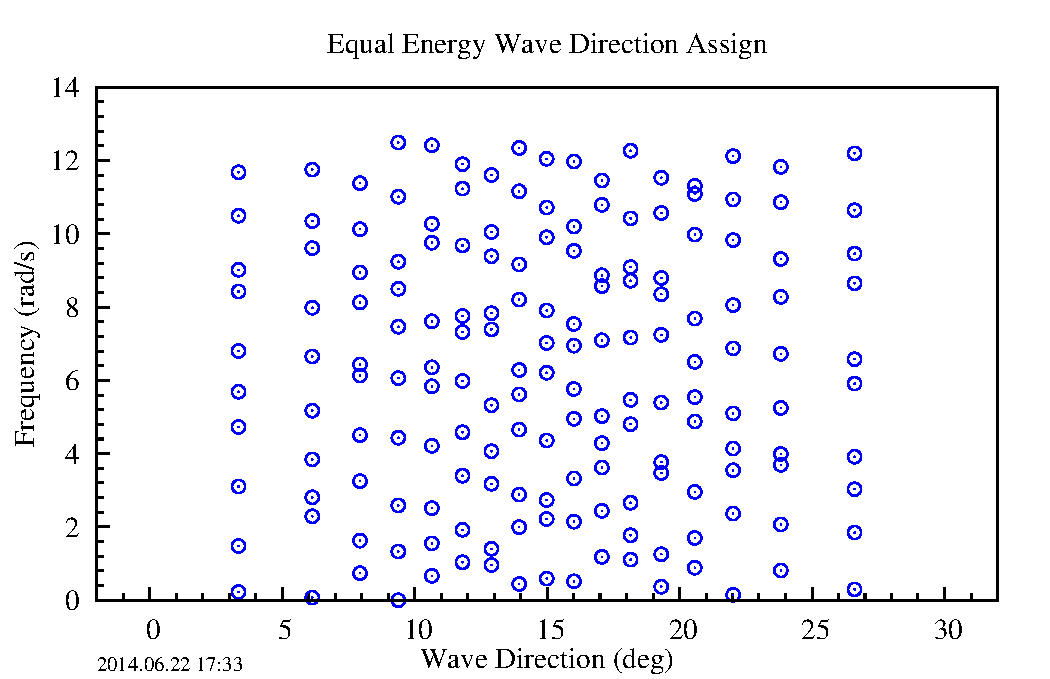
\includegraphics[width=.47\linewidth]{chaps/figures/WaveDirTest/WavesTest_008--wavedir_assign.pdf}
   \caption{Test case 008.  The right plot shows the randomly selected directions for each frequency.\label{fig:MultiDir:WavesTest008}}
\end{figure}



%\section{Modifications to wave velocity and acceleration equations}
%\label{sec:MultiDir:eqMods}
%
%Several of the equations used within the \modname{Waves} module are modified to accomodate the wavedirections as a function of frequency.  In Jason's dissertation, the $cos(\beta)$ and $sin(\beta)$ terms in equation 2-31a, 2-31b, 2-32a, and 2-32b are moved inside the IFFT.  %In the code, these are now implimented as %page 33 of dissertation 
%\begin{equation}
%v_1(t,X,Y,Z) = 
%\label{eq:MultiDir:WaveVelxi}
%\end{equation}


\clearpage
\section{Changes during implimentation}
\begin{description}
   \item[Waves module:]{\varname{InitOutputType\%WaveDir} will continue to contain the mean wave heading.  A new array \varname{InitOutputType\%WaveDirArr} will contain the direction headings for each wave elevation (same number of elements as \varname{WaveElevCO}).}
   \item[Waves module:]{For calculations of wave height, velocity, and acceleration away from the origin, modifications were made to split the wave into $x$ and $y$ components and calculate each separately (used to be single component along wave direction).}
   \item[Waves module:]{the equations for the wave velocity and acceleration used within the \modname{Waves} module are modified to accomodate the wavedirections as a function of frequency.  In Jason's dissertation, the $cos(\beta)$ and $sin(\beta)$ terms in equation 2-31a, 2-31b, 2-32a, and 2-32b are moved inside the IFFT.}  %In the code, these are now implimented as %page 33 of dissertation}
   \item[WAMIT module:]{Change wording about \varname{WaveDir} to correspond to the mean wave direction.  Add in a new variable \varname{WaveDirArr} to handle the directions for each frequency.}
   \item[WAMIT module:]{Change the code to use \varname{WaveDirArr} at each frequency.  This involved combining what had been two one-dimensional interpolations into a single two-dimensional interpolation scheme.}
\end{description}

In addition to the above changes, a new pair of input and output arrays were specified to allow for the calculation of the wave elevation at arbitrarily specified (X,Y) coordinates.  The input array, \varname{WaveElevXY}, of size $2\times N$ allows the for a set of $N$ arbitrary number of $(x,y)$ coordinates to be specified.  For this array, index 1 corresponds to specifies which coordinate ($x$ or $y$) and index 2 corresponds to point number.  If \varname{WaveElevXY} has been allocated at the gluecode or driver level, an array, \varname{WaveElevSeries}, of size \varname{NStepWave}$\times N$ is returned.  The first index of this array is the timestep (of the \varname{NStepWave} timesteps in the simulation), and the second index corresponds to the point number (of $N$ points) specified in the \varname{WaveElevXY} input array.  This has been implimented both within the \modname{Waves} module and within \HD itself.  It has been tested with the \HD driver and with the \modname{WAMIT2} driver code to generate sea surface movies corresponding to each of the 8 tests listed in \Cref{tab:MultiDir:Tests}.
